\documentclass[tikz,border=8pt]{standalone}
\usepackage[utf8]{inputenc}
\usepackage[T1]{fontenc}

\usepackage{amsmath}
\usetikzlibrary{arrows.meta, positioning, calc, fit}
\renewcommand{\familydefault}{\sfdefault}
\begin{document}
	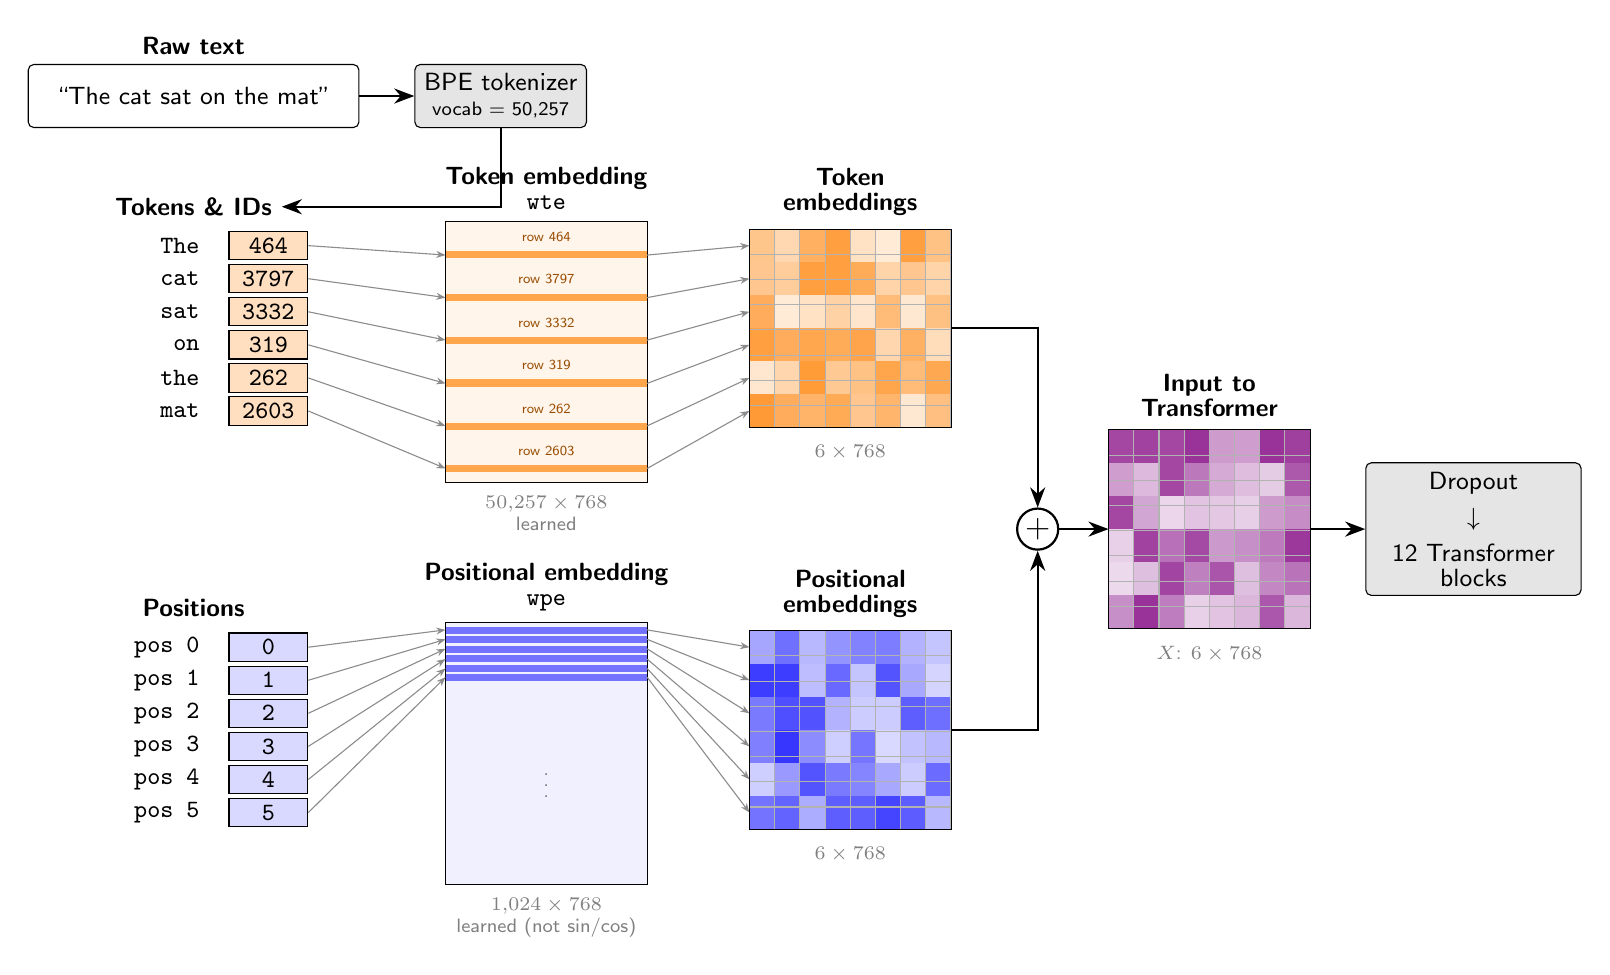
\begin{tikzpicture}[
		arrow/.style={-{Stealth[scale=1.1]}, thick},
		lk/.style={-{Stealth[scale=0.7]}, black!45},
		ttl/.style={font=\sffamily\small\bfseries, anchor=south, align=center},
		sub/.style={font=\sffamily\scriptsize, text=gray, anchor=north, align=center},
		box/.style={rectangle, rounded corners=2pt, draw=black, fill=gray!12, font=\sffamily\small, align=center, minimum height=0.8cm}
		]
		\node[box, fill=white, minimum width=4.2cm] (text) at (0.4,1.9) {\textquotedblleft The cat sat on the mat\textquotedblright};
		\node[ttl] at (text.north) {Raw text};
		\node[box, fill=gray!20] (tok) at (4.3,1.9) {BPE tokenizer\\[-2pt]{\scriptsize vocab = 50{,}257}};
		\draw[arrow] (text) -- (tok);
		\node[anchor=east, font=\ttfamily\small] at (0.60,0.00) {The};
		\node[draw, fill=orange!25, minimum width=1.0cm, minimum height=0.36cm, font=\ttfamily\small, inner sep=1pt] (id0) at (1.35,0.00) {464};
		\node[anchor=east, font=\ttfamily\small] at (0.60,-0.42) {cat};
		\node[draw, fill=orange!25, minimum width=1.0cm, minimum height=0.36cm, font=\ttfamily\small, inner sep=1pt] (id1) at (1.35,-0.42) {3797};
		\node[anchor=east, font=\ttfamily\small] at (0.60,-0.84) {sat};
		\node[draw, fill=orange!25, minimum width=1.0cm, minimum height=0.36cm, font=\ttfamily\small, inner sep=1pt] (id2) at (1.35,-0.84) {3332};
		\node[anchor=east, font=\ttfamily\small] at (0.60,-1.26) {on};
		\node[draw, fill=orange!25, minimum width=1.0cm, minimum height=0.36cm, font=\ttfamily\small, inner sep=1pt] (id3) at (1.35,-1.26) {319};
		\node[anchor=east, font=\ttfamily\small] at (0.60,-1.68) {the};
		\node[draw, fill=orange!25, minimum width=1.0cm, minimum height=0.36cm, font=\ttfamily\small, inner sep=1pt] (id4) at (1.35,-1.68) {262};
		\node[anchor=east, font=\ttfamily\small] at (0.60,-2.10) {mat};
		\node[draw, fill=orange!25, minimum width=1.0cm, minimum height=0.36cm, font=\ttfamily\small, inner sep=1pt] (id5) at (1.35,-2.10) {2603};
		\node[ttl] (tidt) at (0.4,0.26) {Tokens \& IDs};
		\draw[arrow] (tok.south) |- (tidt.east);
		\draw[fill=orange!8] (3.6,0.31) rectangle ++(2.56,-3.32);
		\fill[orange!70] (3.6,-0.07) rectangle ++(2.56,-0.09);
		\coordinate (wte0) at (3.6,-0.12);
		\coordinate (wteo0) at (6.16,-0.12);
		\draw[lk] (id0.east) -- (wte0);
		\node[font=\sffamily\tiny, text=orange!60!black, anchor=south] at (4.88,-0.07) {row 464};
		\fill[orange!70] (3.6,-0.61) rectangle ++(2.56,-0.09);
		\coordinate (wte1) at (3.6,-0.66);
		\coordinate (wteo1) at (6.16,-0.66);
		\draw[lk] (id1.east) -- (wte1);
		\node[font=\sffamily\tiny, text=orange!60!black, anchor=south] at (4.88,-0.61) {row 3797};
		\fill[orange!70] (3.6,-1.16) rectangle ++(2.56,-0.09);
		\coordinate (wte2) at (3.6,-1.20);
		\coordinate (wteo2) at (6.16,-1.20);
		\draw[lk] (id2.east) -- (wte2);
		\node[font=\sffamily\tiny, text=orange!60!black, anchor=south] at (4.88,-1.16) {row 3332};
		\fill[orange!70] (3.6,-1.70) rectangle ++(2.56,-0.09);
		\coordinate (wte3) at (3.6,-1.75);
		\coordinate (wteo3) at (6.16,-1.75);
		\draw[lk] (id3.east) -- (wte3);
		\node[font=\sffamily\tiny, text=orange!60!black, anchor=south] at (4.88,-1.70) {row 319};
		\fill[orange!70] (3.6,-2.25) rectangle ++(2.56,-0.09);
		\coordinate (wte4) at (3.6,-2.29);
		\coordinate (wteo4) at (6.16,-2.29);
		\draw[lk] (id4.east) -- (wte4);
		\node[font=\sffamily\tiny, text=orange!60!black, anchor=south] at (4.88,-2.25) {row 262};
		\fill[orange!70] (3.6,-2.79) rectangle ++(2.56,-0.09);
		\coordinate (wte5) at (3.6,-2.83);
		\coordinate (wteo5) at (6.16,-2.83);
		\draw[lk] (id5.east) -- (wte5);
		\node[font=\sffamily\tiny, text=orange!60!black, anchor=south] at (4.88,-2.79) {row 2603};
		\node[ttl] at (4.88,0.33) {Token embedding\\[-2pt]\texttt{wte}};
		\node[sub] at (4.88,-3.06) {$50{,}257 \times 768$\\learned};
		\fill[orange!45!white] (7.46,0.21) rectangle ++(0.32,-0.42);
		\fill[orange!31!white] (7.78,0.21) rectangle ++(0.32,-0.42);
		\fill[orange!62!white] (8.10,0.21) rectangle ++(0.32,-0.42);
		\fill[orange!75!white] (8.42,0.21) rectangle ++(0.32,-0.42);
		\fill[orange!23!white] (8.74,0.21) rectangle ++(0.32,-0.42);
		\fill[orange!16!white] (9.06,0.21) rectangle ++(0.32,-0.42);
		\fill[orange!75!white] (9.38,0.21) rectangle ++(0.32,-0.42);
		\fill[orange!48!white] (9.70,0.21) rectangle ++(0.32,-0.42);
		\coordinate (e0) at (7.46,0.00);
		\fill[orange!44!white] (7.46,-0.21) rectangle ++(0.32,-0.42);
		\fill[orange!39!white] (7.78,-0.21) rectangle ++(0.32,-0.42);
		\fill[orange!75!white] (8.10,-0.21) rectangle ++(0.32,-0.42);
		\fill[orange!75!white] (8.42,-0.21) rectangle ++(0.32,-0.42);
		\fill[orange!65!white] (8.74,-0.21) rectangle ++(0.32,-0.42);
		\fill[orange!34!white] (9.06,-0.21) rectangle ++(0.32,-0.42);
		\fill[orange!44!white] (9.38,-0.21) rectangle ++(0.32,-0.42);
		\fill[orange!34!white] (9.70,-0.21) rectangle ++(0.32,-0.42);
		\coordinate (e1) at (7.46,-0.42);
		\fill[orange!64!white] (7.46,-0.63) rectangle ++(0.32,-0.42);
		\fill[orange!16!white] (7.78,-0.63) rectangle ++(0.32,-0.42);
		\fill[orange!23!white] (8.10,-0.63) rectangle ++(0.32,-0.42);
		\fill[orange!35!white] (8.42,-0.63) rectangle ++(0.32,-0.42);
		\fill[orange!20!white] (8.74,-0.63) rectangle ++(0.32,-0.42);
		\fill[orange!53!white] (9.06,-0.63) rectangle ++(0.32,-0.42);
		\fill[orange!18!white] (9.38,-0.63) rectangle ++(0.32,-0.42);
		\fill[orange!49!white] (9.70,-0.63) rectangle ++(0.32,-0.42);
		\coordinate (e2) at (7.46,-0.84);
		\fill[orange!75!white] (7.46,-1.05) rectangle ++(0.32,-0.42);
		\fill[orange!64!white] (7.78,-1.05) rectangle ++(0.32,-0.42);
		\fill[orange!69!white] (8.10,-1.05) rectangle ++(0.32,-0.42);
		\fill[orange!65!white] (8.42,-1.05) rectangle ++(0.32,-0.42);
		\fill[orange!71!white] (8.74,-1.05) rectangle ++(0.32,-0.42);
		\fill[orange!32!white] (9.06,-1.05) rectangle ++(0.32,-0.42);
		\fill[orange!61!white] (9.38,-1.05) rectangle ++(0.32,-0.42);
		\fill[orange!27!white] (9.70,-1.05) rectangle ++(0.32,-0.42);
		\coordinate (e3) at (7.46,-1.26);
		\fill[orange!19!white] (7.46,-1.47) rectangle ++(0.32,-0.42);
		\fill[orange!32!white] (7.78,-1.47) rectangle ++(0.32,-0.42);
		\fill[orange!78!white] (8.10,-1.47) rectangle ++(0.32,-0.42);
		\fill[orange!42!white] (8.42,-1.47) rectangle ++(0.32,-0.42);
		\fill[orange!48!white] (8.74,-1.47) rectangle ++(0.32,-0.42);
		\fill[orange!70!white] (9.06,-1.47) rectangle ++(0.32,-0.42);
		\fill[orange!53!white] (9.38,-1.47) rectangle ++(0.32,-0.42);
		\fill[orange!68!white] (9.70,-1.47) rectangle ++(0.32,-0.42);
		\coordinate (e4) at (7.46,-1.68);
		\fill[orange!79!white] (7.46,-1.89) rectangle ++(0.32,-0.42);
		\fill[orange!64!white] (7.78,-1.89) rectangle ++(0.32,-0.42);
		\fill[orange!59!white] (8.10,-1.89) rectangle ++(0.32,-0.42);
		\fill[orange!67!white] (8.42,-1.89) rectangle ++(0.32,-0.42);
		\fill[orange!44!white] (8.74,-1.89) rectangle ++(0.32,-0.42);
		\fill[orange!58!white] (9.06,-1.89) rectangle ++(0.32,-0.42);
		\fill[orange!18!white] (9.38,-1.89) rectangle ++(0.32,-0.42);
		\fill[orange!50!white] (9.70,-1.89) rectangle ++(0.32,-0.42);
		\coordinate (e5) at (7.46,-2.10);
		\draw[step=0.32, black!30, xshift=7.46cm, yshift=0.21cm] (0,0) grid (2.56,-2.52);
		\draw (7.46,0.21) rectangle ++(2.56,-2.52);
		\node[sub] at (8.74,-2.41) {$6 \times 768$};
		\coordinate (eE) at (10.02,-1.05);
		\coordinate (eW) at (7.46,-1.05);
		\draw[lk] (wteo0) -- (e0);
		\draw[lk] (wteo1) -- (e1);
		\draw[lk] (wteo2) -- (e2);
		\draw[lk] (wteo3) -- (e3);
		\draw[lk] (wteo4) -- (e4);
		\draw[lk] (wteo5) -- (e5);
		\node[ttl] at (8.74,0.26) {Token\\[-2pt]embeddings};
		\node[anchor=east, font=\ttfamily\small] at (0.60,-5.10) {pos 0};
		\node[draw, fill=blue!15, minimum width=1.0cm, minimum height=0.36cm, font=\ttfamily\small, inner sep=1pt] (p0) at (1.35,-5.10) {0};
		\node[anchor=east, font=\ttfamily\small] at (0.60,-5.52) {pos 1};
		\node[draw, fill=blue!15, minimum width=1.0cm, minimum height=0.36cm, font=\ttfamily\small, inner sep=1pt] (p1) at (1.35,-5.52) {1};
		\node[anchor=east, font=\ttfamily\small] at (0.60,-5.94) {pos 2};
		\node[draw, fill=blue!15, minimum width=1.0cm, minimum height=0.36cm, font=\ttfamily\small, inner sep=1pt] (p2) at (1.35,-5.94) {2};
		\node[anchor=east, font=\ttfamily\small] at (0.60,-6.36) {pos 3};
		\node[draw, fill=blue!15, minimum width=1.0cm, minimum height=0.36cm, font=\ttfamily\small, inner sep=1pt] (p3) at (1.35,-6.36) {3};
		\node[anchor=east, font=\ttfamily\small] at (0.60,-6.78) {pos 4};
		\node[draw, fill=blue!15, minimum width=1.0cm, minimum height=0.36cm, font=\ttfamily\small, inner sep=1pt] (p4) at (1.35,-6.78) {4};
		\node[anchor=east, font=\ttfamily\small] at (0.60,-7.20) {pos 5};
		\node[draw, fill=blue!15, minimum width=1.0cm, minimum height=0.36cm, font=\ttfamily\small, inner sep=1pt] (p5) at (1.35,-7.20) {5};
		\node[ttl] at (0.4,-4.84) {Positions};
		\draw[fill=blue!6] (3.6,-4.79) rectangle ++(2.56,-3.32);
		\fill[blue!55] (3.6,-4.84) rectangle ++(2.56,-0.09);
		\draw[lk] (p0.east) -- (3.6,-4.88);
		\draw[lk] (6.16,-4.88) -- (7.46,-5.10);
		\fill[blue!55] (3.6,-4.96) rectangle ++(2.56,-0.09);
		\draw[lk] (p1.east) -- (3.6,-5.00);
		\draw[lk] (6.16,-5.00) -- (7.46,-5.52);
		\fill[blue!55] (3.6,-5.08) rectangle ++(2.56,-0.09);
		\draw[lk] (p2.east) -- (3.6,-5.12);
		\draw[lk] (6.16,-5.12) -- (7.46,-5.94);
		\fill[blue!55] (3.6,-5.20) rectangle ++(2.56,-0.09);
		\draw[lk] (p3.east) -- (3.6,-5.25);
		\draw[lk] (6.16,-5.25) -- (7.46,-6.36);
		\fill[blue!55] (3.6,-5.32) rectangle ++(2.56,-0.09);
		\draw[lk] (p4.east) -- (3.6,-5.37);
		\draw[lk] (6.16,-5.37) -- (7.46,-6.78);
		\fill[blue!55] (3.6,-5.44) rectangle ++(2.56,-0.09);
		\draw[lk] (p5.east) -- (3.6,-5.48);
		\draw[lk] (6.16,-5.48) -- (7.46,-7.20);
		\node[font=\sffamily\scriptsize, text=gray] at (4.88,-6.75) {$\vdots$};
		\node[ttl] at (4.88,-4.77) {Positional embedding\\[-2pt]\texttt{wpe}};
		\node[sub] at (4.88,-8.16) {$1{,}024 \times 768$\\learned (not sin/cos)};
		\fill[blue!35!white] (7.46,-4.89) rectangle ++(0.32,-0.42);
		\fill[blue!56!white] (7.78,-4.89) rectangle ++(0.32,-0.42);
		\fill[blue!28!white] (8.10,-4.89) rectangle ++(0.32,-0.42);
		\fill[blue!42!white] (8.42,-4.89) rectangle ++(0.32,-0.42);
		\fill[blue!49!white] (8.74,-4.89) rectangle ++(0.32,-0.42);
		\fill[blue!51!white] (9.06,-4.89) rectangle ++(0.32,-0.42);
		\fill[blue!30!white] (9.38,-4.89) rectangle ++(0.32,-0.42);
		\fill[blue!23!white] (9.70,-4.89) rectangle ++(0.32,-0.42);
		\coordinate (q0) at (7.46,-5.10);
		\fill[blue!76!white] (7.46,-5.31) rectangle ++(0.32,-0.42);
		\fill[blue!76!white] (7.78,-5.31) rectangle ++(0.32,-0.42);
		\fill[blue!26!white] (8.10,-5.31) rectangle ++(0.32,-0.42);
		\fill[blue!59!white] (8.42,-5.31) rectangle ++(0.32,-0.42);
		\fill[blue!23!white] (8.74,-5.31) rectangle ++(0.32,-0.42);
		\fill[blue!67!white] (9.06,-5.31) rectangle ++(0.32,-0.42);
		\fill[blue!34!white] (9.38,-5.31) rectangle ++(0.32,-0.42);
		\fill[blue!17!white] (9.70,-5.31) rectangle ++(0.32,-0.42);
		\coordinate (q1) at (7.46,-5.52);
		\fill[blue!52!white] (7.46,-5.73) rectangle ++(0.32,-0.42);
		\fill[blue!69!white] (7.78,-5.73) rectangle ++(0.32,-0.42);
		\fill[blue!68!white] (8.10,-5.73) rectangle ++(0.32,-0.42);
		\fill[blue!30!white] (8.42,-5.73) rectangle ++(0.32,-0.42);
		\fill[blue!20!white] (8.74,-5.73) rectangle ++(0.32,-0.42);
		\fill[blue!20!white] (9.06,-5.73) rectangle ++(0.32,-0.42);
		\fill[blue!63!white] (9.38,-5.73) rectangle ++(0.32,-0.42);
		\fill[blue!57!white] (9.70,-5.73) rectangle ++(0.32,-0.42);
		\coordinate (q2) at (7.46,-5.94);
		\fill[blue!50!white] (7.46,-6.15) rectangle ++(0.32,-0.42);
		\fill[blue!79!white] (7.78,-6.15) rectangle ++(0.32,-0.42);
		\fill[blue!45!white] (8.10,-6.15) rectangle ++(0.32,-0.42);
		\fill[blue!19!white] (8.42,-6.15) rectangle ++(0.32,-0.42);
		\fill[blue!54!white] (8.74,-6.15) rectangle ++(0.32,-0.42);
		\fill[blue!15!white] (9.06,-6.15) rectangle ++(0.32,-0.42);
		\fill[blue!24!white] (9.38,-6.15) rectangle ++(0.32,-0.42);
		\fill[blue!28!white] (9.70,-6.15) rectangle ++(0.32,-0.42);
		\coordinate (q3) at (7.46,-6.36);
		\fill[blue!19!white] (7.46,-6.57) rectangle ++(0.32,-0.42);
		\fill[blue!40!white] (7.78,-6.57) rectangle ++(0.32,-0.42);
		\fill[blue!67!white] (8.10,-6.57) rectangle ++(0.32,-0.42);
		\fill[blue!52!white] (8.42,-6.57) rectangle ++(0.32,-0.42);
		\fill[blue!48!white] (8.74,-6.57) rectangle ++(0.32,-0.42);
		\fill[blue!34!white] (9.06,-6.57) rectangle ++(0.32,-0.42);
		\fill[blue!20!white] (9.38,-6.57) rectangle ++(0.32,-0.42);
		\fill[blue!58!white] (9.70,-6.57) rectangle ++(0.32,-0.42);
		\coordinate (q4) at (7.46,-6.78);
		\fill[blue!55!white] (7.46,-6.99) rectangle ++(0.32,-0.42);
		\fill[blue!61!white] (7.78,-6.99) rectangle ++(0.32,-0.42);
		\fill[blue!32!white] (8.10,-6.99) rectangle ++(0.32,-0.42);
		\fill[blue!63!white] (8.42,-6.99) rectangle ++(0.32,-0.42);
		\fill[blue!63!white] (8.74,-6.99) rectangle ++(0.32,-0.42);
		\fill[blue!73!white] (9.06,-6.99) rectangle ++(0.32,-0.42);
		\fill[blue!64!white] (9.38,-6.99) rectangle ++(0.32,-0.42);
		\fill[blue!28!white] (9.70,-6.99) rectangle ++(0.32,-0.42);
		\coordinate (q5) at (7.46,-7.20);
		\draw[step=0.32, black!30, xshift=7.46cm, yshift=-4.89cm] (0,0) grid (2.56,-2.52);
		\draw (7.46,-4.89) rectangle ++(2.56,-2.52);
		\node[sub] at (8.74,-7.51) {$6 \times 768$};
		\coordinate (qE) at (10.02,-6.15);
		\coordinate (qW) at (7.46,-6.15);
		\node[ttl] at (8.74,-4.84) {Positional\\[-2pt]embeddings};
		\node[circle, draw, thick, inner sep=1pt, font=\large] (plus) at (11.12,-3.60) {$+$};
		\draw[arrow] (eE) -| (plus.north);
		\draw[arrow] (qE) -| (plus.south);
		\fill[violet!72!white] (12.02,-2.34) rectangle ++(0.32,-0.42);
		\fill[violet!74!white] (12.34,-2.34) rectangle ++(0.32,-0.42);
		\fill[violet!72!white] (12.66,-2.34) rectangle ++(0.32,-0.42);
		\fill[violet!80!white] (12.98,-2.34) rectangle ++(0.32,-0.42);
		\fill[violet!39!white] (13.30,-2.34) rectangle ++(0.32,-0.42);
		\fill[violet!38!white] (13.62,-2.34) rectangle ++(0.32,-0.42);
		\fill[violet!80!white] (13.94,-2.34) rectangle ++(0.32,-0.42);
		\fill[violet!75!white] (14.26,-2.34) rectangle ++(0.32,-0.42);
		\coordinate (x0) at (12.02,-2.55);
		\fill[violet!38!white] (12.02,-2.76) rectangle ++(0.32,-0.42);
		\fill[violet!27!white] (12.34,-2.76) rectangle ++(0.32,-0.42);
		\fill[violet!72!white] (12.66,-2.76) rectangle ++(0.32,-0.42);
		\fill[violet!53!white] (12.98,-2.76) rectangle ++(0.32,-0.42);
		\fill[violet!33!white] (13.30,-2.76) rectangle ++(0.32,-0.42);
		\fill[violet!26!white] (13.62,-2.76) rectangle ++(0.32,-0.42);
		\fill[violet!20!white] (13.94,-2.76) rectangle ++(0.32,-0.42);
		\fill[violet!65!white] (14.26,-2.76) rectangle ++(0.32,-0.42);
		\coordinate (x1) at (12.02,-2.97);
		\fill[violet!72!white] (12.02,-3.18) rectangle ++(0.32,-0.42);
		\fill[violet!35!white] (12.34,-3.18) rectangle ++(0.32,-0.42);
		\fill[violet!16!white] (12.66,-3.18) rectangle ++(0.32,-0.42);
		\fill[violet!23!white] (12.98,-3.18) rectangle ++(0.32,-0.42);
		\fill[violet!22!white] (13.30,-3.18) rectangle ++(0.32,-0.42);
		\fill[violet!19!white] (13.62,-3.18) rectangle ++(0.32,-0.42);
		\fill[violet!39!white] (13.94,-3.18) rectangle ++(0.32,-0.42);
		\fill[violet!45!white] (14.26,-3.18) rectangle ++(0.32,-0.42);
		\coordinate (x2) at (12.02,-3.39);
		\fill[violet!18!white] (12.02,-3.60) rectangle ++(0.32,-0.42);
		\fill[violet!74!white] (12.34,-3.60) rectangle ++(0.32,-0.42);
		\fill[violet!56!white] (12.66,-3.60) rectangle ++(0.32,-0.42);
		\fill[violet!71!white] (12.98,-3.60) rectangle ++(0.32,-0.42);
		\fill[violet!40!white] (13.30,-3.60) rectangle ++(0.32,-0.42);
		\fill[violet!44!white] (13.62,-3.60) rectangle ++(0.32,-0.42);
		\fill[violet!52!white] (13.94,-3.60) rectangle ++(0.32,-0.42);
		\fill[violet!78!white] (14.26,-3.60) rectangle ++(0.32,-0.42);
		\coordinate (x3) at (12.02,-3.81);
		\fill[violet!15!white] (12.02,-4.02) rectangle ++(0.32,-0.42);
		\fill[violet!25!white] (12.34,-4.02) rectangle ++(0.32,-0.42);
		\fill[violet!73!white] (12.66,-4.02) rectangle ++(0.32,-0.42);
		\fill[violet!50!white] (12.98,-4.02) rectangle ++(0.32,-0.42);
		\fill[violet!67!white] (13.30,-4.02) rectangle ++(0.32,-0.42);
		\fill[violet!25!white] (13.62,-4.02) rectangle ++(0.32,-0.42);
		\fill[violet!47!white] (13.94,-4.02) rectangle ++(0.32,-0.42);
		\fill[violet!55!white] (14.26,-4.02) rectangle ++(0.32,-0.42);
		\coordinate (x4) at (12.02,-4.23);
		\fill[violet!44!white] (12.02,-4.44) rectangle ++(0.32,-0.42);
		\fill[violet!80!white] (12.34,-4.44) rectangle ++(0.32,-0.42);
		\fill[violet!51!white] (12.66,-4.44) rectangle ++(0.32,-0.42);
		\fill[violet!18!white] (12.98,-4.44) rectangle ++(0.32,-0.42);
		\fill[violet!23!white] (13.30,-4.44) rectangle ++(0.32,-0.42);
		\fill[violet!28!white] (13.62,-4.44) rectangle ++(0.32,-0.42);
		\fill[violet!66!white] (13.94,-4.44) rectangle ++(0.32,-0.42);
		\fill[violet!28!white] (14.26,-4.44) rectangle ++(0.32,-0.42);
		\coordinate (x5) at (12.02,-4.65);
		\draw[step=0.32, black!30, xshift=12.02cm, yshift=-2.34cm] (0,0) grid (2.56,-2.52);
		\draw (12.02,-2.34) rectangle ++(2.56,-2.52);
		\node[sub] at (13.30,-4.96) {$X$: $6 \times 768$};
		\coordinate (xE) at (14.58,-3.60);
		\coordinate (xW) at (12.02,-3.60);
		\node[ttl] at (13.30,-2.29) {Input to\\[-2pt]Transformer};
		\draw[arrow] (plus.east) -- (xW);
		\node[box, fill=gray!20, right=0.7cm of xE, minimum height=1.6cm, text width=2.5cm] (blocks) {Dropout\\[2pt]$\downarrow$\\[2pt]12 Transformer\\[-2pt]blocks};
		\draw[arrow] (xE) -- (blocks);
	\end{tikzpicture}
\end{document}